\documentclass[a4paper,12pt]{article}
\usepackage{color}
\usepackage{graphicx}
\begin{document}

\title{\textbf{NGspice And geda Schematic}}
\author{Shelcia Carolyn Samuvel}
\date{\today}
\maketitle

\pagenumbering{roman}
\tableofcontents
\newpage
\pagenumbering{arabic}

\section{Introduction}
This document is to show how to use \textbf{NGspice} and \textbf{geda} to analyze circuits and produce outputs.

\section{Installation}
Lets install both the required software in the system before we proceed. Since the project has been done on a Linux system, It will be assumed that the user is operating a Linux OS, preferably Ubuntu.

Type the following commands in the terminal to install the packages:
{\color{red}sudo apt install ngspice}

{\color{red}sudo apt install geda}



\newpage

\section{Schematic}

The first step is to prepare a working schematic. To achieve this open \textbf{gschem}.Draw the schematic with the required components and the values as shown in figure.

\begin{figure}[h!]
\centering
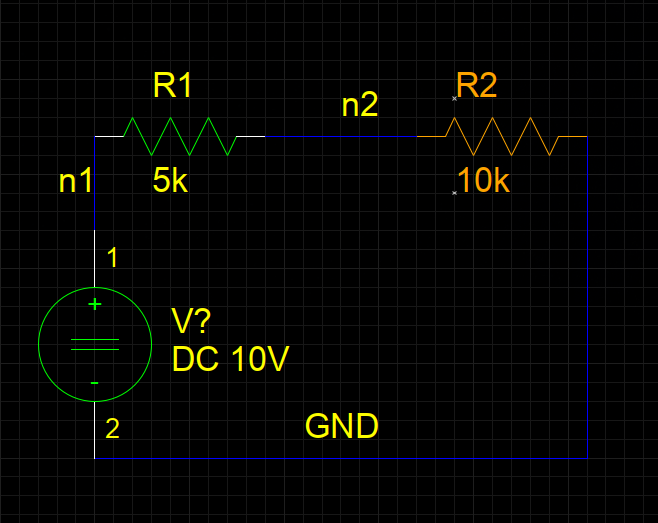
\includegraphics[width=1\textwidth]{Schematic.png}
\caption{Schematic}
\end{figure}

\newpage

\section{Generating the netlist}
The commands in the terminal are shown in the image below:

\begin{figure}[h!]
\centering
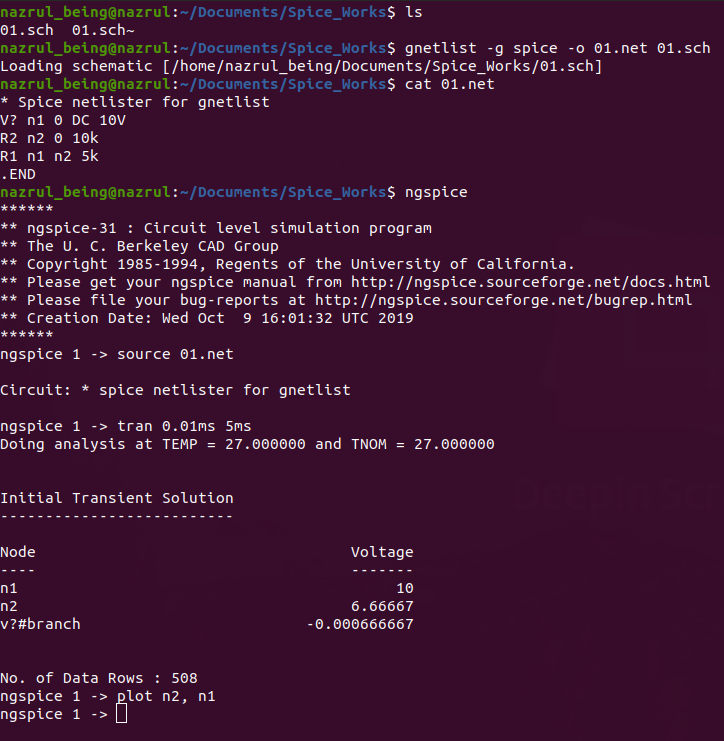
\includegraphics[width=1\textwidth]{Terminal.png}
\caption{Generating the netlist}
\end{figure}

Under the part of \textbf{Initial Transient Solution} we have obtained some values. We plot the graph using this values to see what is happening with the circuit.


\section{Plot}
After performing all commands, as described in the previous section (Generating the netlist) we plot the graph. We can see we obtain a graph similar to this.

\begin{figure}[h!]
\centering
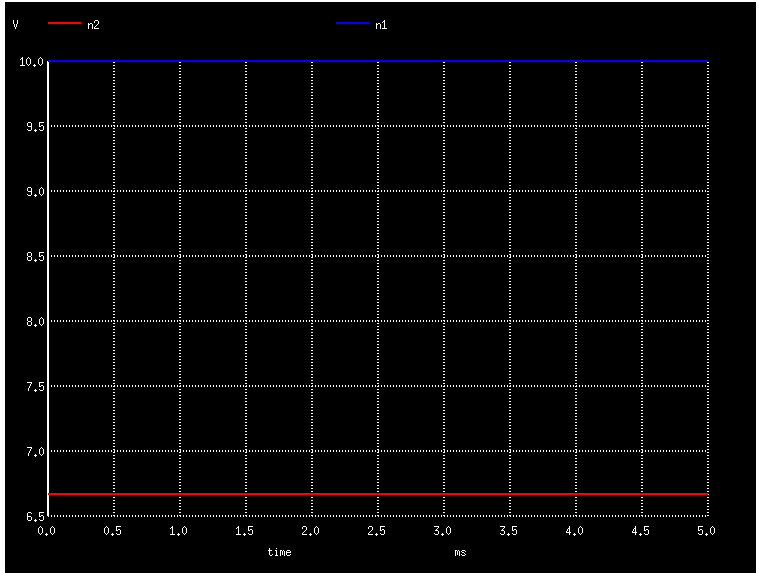
\includegraphics[width=1\textwidth]{plot.png}
\caption{Plot}
\end{figure}

\newpage

\section{Result}
This method of analyzing circuits is much easier and accurate. As we can see that the circuit is a simple voltage divider. Using this form of analysis gives us much better understanding of circuits and at the same time allows us to solve the circuits with much less effort and accurately.\\\\\\\\

\centering
\textbf{Thank You!}

\end{document}
